
In order to understand the motivations, limitations and behaviour of the experiment we need to know about a few key concepts in fluid dynamics.

\subsection{Navier Stokes}


\subsection{Reynold's Number}
The Reynolds number (Re) is a dimensionless number describing the ratio of inertial forces to viscous forces in a flow. For flow in a pipe it is defined as \cite{introfluid}

\begin{equation}\label{eq:reynolds}
Re = \frac{U L \rho}{\mu}
\end{equation}
where $U$ is the characteristic velocity of the flow, $L$ is the characteristic length, $\rho$ is the density and $\mu$ is the dynamic viscosity. This is used to estimate the 'regime' of the flow, of which there are two primary types. 
\begin{enumerate}
\item Laminar flow, where viscous forces dominate over inertial forces
\item Turbulent regime where inertial forces dominate.
\end{enumerate}

As the Reynolds number is a ratio between the inertial forces and viscous forces we get more turbulent flow for larger Reynolds numbers, a simple visual characterization of the flow types can be seen in figure \ref{fig:laminar_flow}. For $operatorname{Re}\ll 1$ it is referred to as \emph{Stokes flow} and we can ignore intertial forces completely. This actually means that not only is the flow completely guaranteed to be laminar, but it is time reversible, meaning that reversing the flow any dynamics of the flow and particles in the flow will revert perfectly as well \cite{introfluid3}.

\begin{figure}[H]
\centering
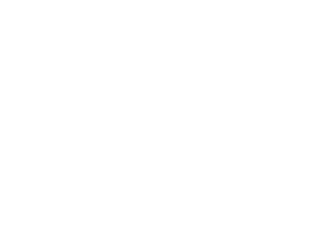
\includegraphics[width=\textwidth]{figures/theory/laminarFlow.pdf}
\caption{This shows the principal difference between laminar and turbulent flow}
\label{fig:laminar_flow}
\end{figure}


\subsection{Stokes Drag and Stokes's law}
The drag force $F_D$ exerted by a fluid on a spherical particle for $Re << 1$ is found using the so called Stokes's law \cite{introfluid2}

\begin{equation}
F_D = 6\pi \mu R v
\end{equation}

where $v$ is the velocity of the sphere relative to the fluid, $\mu$ is the dynamic viscosity and $R$ is the radius of the sphere. To find the terminal velocity of the sphere we equate this with the gravitational force $F_G$ acting on the sphere

\begin{equation}
F_G = \Delta \rho g\cdot \frac{4\pi R^3}{3}
\end{equation}

where $\Delta \rho$ is the difference in density and $g$ is the specific gravity we find that the terminal velocity of a sinking (or floating) sphere is

\begin{equation}\label{eq:fallingSphere}
v_s = \frac{2}{9} \frac{\Delta \rho}{\mu} g R^2
\end{equation}



%\subsection{Shear}
%
%\subsection{P\'{e}clet Number}
%The p\'{}clet number describes the ratio of thermal noise to other stuff. I really don't know anything about the piclet number.
